\documentclass{beamer}
\usetheme{Boadilla}
\beamertemplatenavigationsymbolsempty
%gets rid of bottom navigation bars
\setbeamertemplate{footline}[page number]{}
%gets rid of navigation symbols
\setbeamertemplate{navigation symbols}{}
\usepackage[latin1]{inputenc}
\usepackage{amsmath,amsfonts,amssymb}
\usepackage{stmaryrd}
\usepackage{tikz}
\usepackage{verbatim}
\usepackage{xcolor}
\usepackage{algorithm}
\usepackage[noend]{algpseudocode}

\setbeamertemplate{caption}{\raggedright\insertcaption\par}

\newlength{\arrowsize}  
\pgfarrowsdeclare{biggertip}{biggertip}{  
  \setlength{\arrowsize}{0.3pt}  
  \addtolength{\arrowsize}{.5\pgflinewidth}  
  \pgfarrowsrightextend{0}  
  \pgfarrowsleftextend{-5\arrowsize}  
}{  
  \setlength{\arrowsize}{0.3pt}  
  \addtolength{\arrowsize}{.5\pgflinewidth}  
  \pgfpathmoveto{\pgfpoint{-5\arrowsize}{4\arrowsize}}  
  \pgfpathlineto{\pgfpointorigin}  
  \pgfpathlineto{\pgfpoint{-5\arrowsize}{-4\arrowsize}}  
  \pgfusepathqstroke  
}  
\newcommand{\redge}[1]{\overset{{}_{\shortleftarrow}}{#1}}
\newcommand{\resedges}[0]{\overset{{}_{\leftrightarrow}}{E}}

\title{Graph algorithmic approach}
\author{Sebastian Schenker}
\date{}

\begin{document}

\frame{\titlepage}

\begin{frame}[fragile]
  \frametitle{Feasibility and optimality}
  \begin{figure}
    \begin{minipage}{0.45\textwidth}
          \caption{Simple instance}
\begin{verbatim}
   4         (time slots)
   2         (types)
   0 1 0 0   (demand)
   0 0 1 1   (demand)
   3         (costs)
   0 4       (costs)
   5 0       (costs)
\end{verbatim}
    \end{minipage}
    \hfill
    \begin{minipage}{0.45\textwidth}
      \begin{itemize}
    \item Feasible schedule:
      \begin{itemize}
      \item demand of each type is fulfilled
      \item at each time slot at most one type is produced
      \end{itemize}
    \item[]
    \item Optimal schedule:
      \begin{itemize}
      \item Lowest cost (inventory + changeover) among all
        feasible schedules
      \end{itemize}
    \end{itemize}
  \end{minipage}
\end{figure}
\end{frame}

\begin{frame}[fragile]
  \frametitle{Feasible schedules}
  \begin{figure}
    \begin{minipage}{0.45\textwidth}
\begin{verbatim}
   0 1 0 0   (demand type 0)
   0 0 1 1   (demand type 1)
\end{verbatim}
    \end{minipage}
    \hfill
    \begin{minipage}{0.45\textwidth}
      \begin{itemize}
      \item 6 feasible schedules:
      \item[] a)~~[ -1 0 1 1 ]
      \item[] b)~~[ 0 -1 1 1 ]
      \item[] c)~~[ 0 1 -1 1 ]
      \item[] d)~~[ 1 0 -1 1 ]
      \item[] e)~~[ 0 1 1 -1 ]
      \item[] f)~~[ 1 0 1 -1 ]
      \end{itemize}
    \end{minipage}
  \end{figure}
\end{frame}

\begin{frame}{Variables}
  \begin{itemize}
  \item consider $x^i_j \in \{0,1\}$ with
  \item[] $x^i_j = 1~\Leftrightarrow$ type $i$ is produced at time
    slot $j$
  \end{itemize}
\end{frame}

\begin{frame}[fragile]
  \frametitle{Graph instance}
  \begin{itemize}
    \item[] \small{0 {\color{red}1} 0 0~~(demand type 0)}
    \item[] \small{0 0 {\color{green}1} {\color{blue}1}~~(demand type 1)}
  \end{itemize}
  \begin{figure}
    \begin{tikzpicture}[transform shape,scale=0.6]
      \useasboundingbox(0,0) rectangle (14,8);
      \tikzset{V/.style = {shape=circle, draw, text=black}}
      \tikzset{E/.style = {draw,text=black,->}}
      \node[V,text=red](d0) at (3,7) {$a$};
      \node[V,text=green](d1) at (7,7) {$b$};
      \node[V,text=blue](d2) at (11,7) {$c$};
      \node[V](x00) at (0,5) {$x^0_0$};
      \node[V](x01) at (2,5) {$x^0_1$};
      \node[V](x02) at (4,5) {$x^0_2$};
      \node[V](x03) at (6,5) {$x^0_3$};
      \node[V](x10) at (8,5) {$x^1_0$};
      \node[V](x11) at (10,5) {$x^1_1$};
      \node[V](x12) at (12,5) {$x^1_2$};
      \node[V](x13) at (14,5) {$x^1_3$};
      \node[V](t0) at (3,3) {$t0$};
      \node[V](t1) at (6,3) {$t1$};
      \node[V](t2) at (9,3) {$t2$};
      \node[V](t3) at (12,3) {$t3$};
      \node[V](t) at (7,1) {\small{$sink$}};
      %% \draw[E](d0) to (x00);
      %% \draw[E](d0) to (x01);
      %% \draw[E](d1) to (x10);
      %% \draw[E](d1) to (x11);
      %% \draw[E](d1) to (x12);
      %% \draw[E](d2) to (x10);
      %% \draw[E](d2) to (x11);
      %% \draw[E](d2) to (x12);
      %% \draw[E](d2) to (x13);
      %% \draw[E](x00) to (t0);
      %% \draw[E](x10) to (t0);
      %% \draw[E](x01) to (t1);
      %% \draw[E](x11) to (t1);
      %% \draw[E](x02) to (t2);
      %% \draw[E](x12) to (t2);
      %% \draw[E](x03) to (t3);
      %% \draw[E](x13) to (t3);
      %% \draw[E](t0) to (t);
      %% \draw[E](t1) to (t);
      %% \draw[E](t2) to (t);
      %% \draw[E](t3) to (t);
      %% \draw[red,->,dashed](3,8) to (d0);
      %% \draw[green,->,dashed](7,8) to (d1);
      %% \draw[blue,->,dashed](11,8) to (d2);
      %% \draw[red,->,dashed](t) to (6.5,0);
      %% \draw[green,->,dashed](t) to (7,0);
      %% \draw[blue,->,dashed](t) to (7.5,0);
    \end{tikzpicture}
  \end{figure}
  \begin{itemize}
  \item Number of vertices: $|\text{items}| + (|\text{time\_slots}| + 1) \cdot |\text{types}| + 1$
  \end{itemize}
\end{frame}

\begin{frame}[fragile]
  \frametitle{Graph instance}
  \begin{itemize}
    \item[] \small{0 {\color{red}1} 0 0~~(demand type 0)}
    \item[] \small{0 0 {\color{green}1} {\color{blue}1}~~(demand type 1)}
  \end{itemize}
  \begin{figure}
    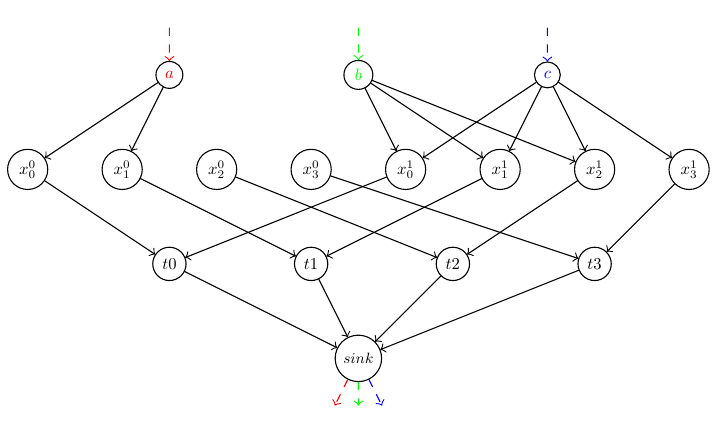
\begin{tikzpicture}[transform shape,scale=0.6]
      \useasboundingbox(0,0) rectangle (14,8);
      \tikzset{V/.style = {shape=circle, draw, text=black}}
      \tikzset{E/.style = {draw,text=black,->}}
      \node[V,text=red](d0) at (3,7) {$a$};
      \node[V,text=green](d1) at (7,7) {$b$};
      \node[V,text=blue](d2) at (11,7) {$c$};
      \node[V](x00) at (0,5) {$x^0_0$};
      \node[V](x01) at (2,5) {$x^0_1$};
      \node[V](x02) at (4,5) {$x^0_2$};
      \node[V](x03) at (6,5) {$x^0_3$};
      \node[V](x10) at (8,5) {$x^1_0$};
      \node[V](x11) at (10,5) {$x^1_1$};
      \node[V](x12) at (12,5) {$x^1_2$};
      \node[V](x13) at (14,5) {$x^1_3$};
      \node[V](t0) at (3,3) {$t0$};
      \node[V](t1) at (6,3) {$t1$};
      \node[V](t2) at (9,3) {$t2$};
      \node[V](t3) at (12,3) {$t3$};
      \node[V](t) at (7,1) {\small{$sink$}};
      \draw[E](d0) to (x00);
      \draw[E](d0) to (x01);
      \draw[E](d1) to (x10);
      \draw[E](d1) to (x11);
      \draw[E](d1) to (x12);
      \draw[E](d2) to (x10);
      \draw[E](d2) to (x11);
      \draw[E](d2) to (x12);
      \draw[E](d2) to (x13);
      \draw[E](x00) to (t0);
      \draw[E](x10) to (t0);
      \draw[E](x01) to (t1);
      \draw[E](x11) to (t1);
      \draw[E](x02) to (t2);
      \draw[E](x12) to (t2);
      \draw[E](x03) to (t3);
      \draw[E](x13) to (t3);
      \draw[E](t0) to (t);
      \draw[E](t1) to (t);
      \draw[E](t2) to (t);
      \draw[E](t3) to (t);
      \draw[red,->,dashed](3,8) to (d0);
      \draw[green,->,dashed](7,8) to (d1);
      \draw[blue,->,dashed](11,8) to (d2);
      \draw[red,->,dashed](t) to (6.5,0);
      \draw[green,->,dashed](t) to (7,0);
      \draw[blue,->,dashed](t) to (7.5,0);
    \end{tikzpicture}
  \end{figure}
  \begin{itemize}
  \item Unit capacity on each edge
  \end{itemize}
\end{frame}

\begin{frame}[fragile]
  \frametitle{Feasible flow corresponds to schedule}
  \begin{figure}
    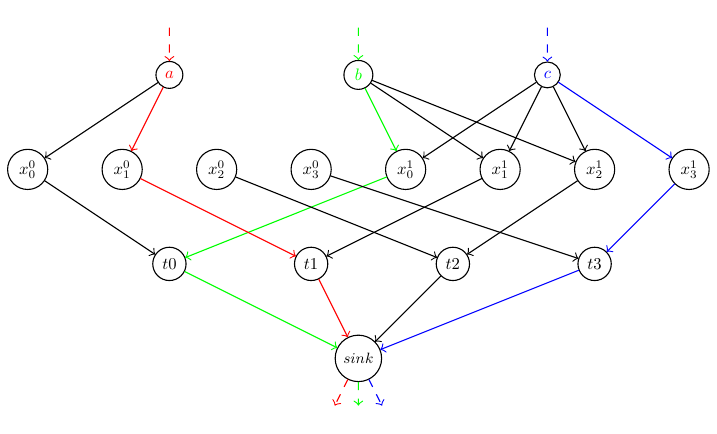
\begin{tikzpicture}[transform shape,scale=0.6]
      \useasboundingbox(0,0) rectangle (14,8);
      \tikzset{V/.style = {shape=circle, draw, text=black}}
      \tikzset{E/.style = {draw,text=black,->}}
      \node[V,text=red](d0) at (3,7) {$a$};
      \node[V,text=green](d1) at (7,7) {$b$};
      \node[V,text=blue](d2) at (11,7) {$c$};
      \node[V](x00) at (0,5) {$x^0_0$};
      \node[V](x01) at (2,5) {$x^0_1$};
      \node[V](x02) at (4,5) {$x^0_2$};
      \node[V](x03) at (6,5) {$x^0_3$};
      \node[V](x10) at (8,5) {$x^1_0$};
      \node[V](x11) at (10,5) {$x^1_1$};
      \node[V](x12) at (12,5) {$x^1_2$};
      \node[V](x13) at (14,5) {$x^1_3$};
      \node[V](t0) at (3,3) {$t0$};
      \node[V](t1) at (6,3) {$t1$};
      \node[V](t2) at (9,3) {$t2$};
      \node[V](t3) at (12,3) {$t3$};
      \node[V](t) at (7,1) {\small{$sink$}};
      \draw[E](d0) to (x00);
      \draw[E,red](d0) to (x01);
      \draw[E,green](d1) to (x10);
      \draw[E](d1) to (x11);
      \draw[E](d1) to (x12);
      \draw[E](d2) to (x10);
      \draw[E](d2) to (x11);
      \draw[E](d2) to (x12);
      \draw[E,blue](d2) to (x13);
      \draw[E](x00) to (t0);
      \draw[E,green](x10) to (t0);
      \draw[E,red](x01) to (t1);
      \draw[E](x11) to (t1);
      \draw[E](x02) to (t2);
      \draw[E](x12) to (t2);
      \draw[E](x03) to (t3);
      \draw[E,blue](x13) to (t3);
      \draw[E,green](t0) to (t);
      \draw[E,red](t1) to (t);
      \draw[E](t2) to (t);
      \draw[E,blue](t3) to (t);
      \draw[red,->,dashed](3,8) to (d0);
      \draw[green,->,dashed](7,8) to (d1);
      \draw[blue,->,dashed](11,8) to (d2);
      \draw[red,->,dashed](t) to (6.5,0);
      \draw[green,->,dashed](t) to (7,0);
      \draw[blue,->,dashed](t) to (7.5,0);
    \end{tikzpicture}
  \end{figure}
  \begin{itemize}
    \item corresponding schedule:  [ 1 0 -1 1 ]
  \end{itemize}
\end{frame}

\begin{frame}[fragile]
  \frametitle{Consider directed cycles in residual graph}
  \begin{figure}
    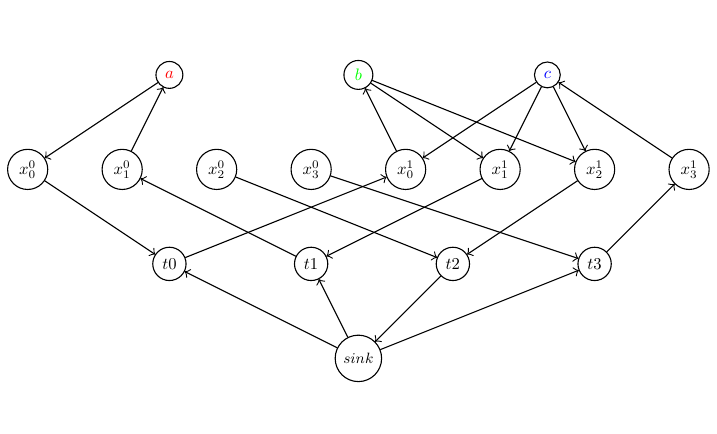
\begin{tikzpicture}[transform shape,scale=0.6]
      \useasboundingbox(0,0) rectangle (14,8);
      \tikzset{V/.style = {shape=circle, draw, text=black}}
      \tikzset{E/.style = {draw,text=black,->}}
      \node[V,text=red](d0) at (3,7) {$a$};
      \node[V,text=green](d1) at (7,7) {$b$};
      \node[V,text=blue](d2) at (11,7) {$c$};
      \node[V](x00) at (0,5) {$x^0_0$};
      \node[V](x01) at (2,5) {$x^0_1$};
      \node[V](x02) at (4,5) {$x^0_2$};
      \node[V](x03) at (6,5) {$x^0_3$};
      \node[V](x10) at (8,5) {$x^1_0$};
      \node[V](x11) at (10,5) {$x^1_1$};
      \node[V](x12) at (12,5) {$x^1_2$};
      \node[V](x13) at (14,5) {$x^1_3$};
      \node[V](t0) at (3,3) {$t0$};
      \node[V](t1) at (6,3) {$t1$};
      \node[V](t2) at (9,3) {$t2$};
      \node[V](t3) at (12,3) {$t3$};
      \node[V](t) at (7,1) {\small{$sink$}};
      \draw[E](d0) to (x00);
      \draw[E] (x01) to (d0);
      \draw[E] (x10) to (d1);
      \draw[E](d1) to (x11);
      \draw[E](d1) to (x12);
      \draw[E](d2) to (x10);
      \draw[E](d2) to (x11);
      \draw[E](d2) to (x12);
      \draw[E] (x13) to (d2);
      \draw[E](x00) to (t0);
      \draw[E] (t0) to (x10);
      \draw[E] (t1) to (x01);
      \draw[E](x11) to (t1);
      \draw[E](x02) to (t2);
      \draw[E](x12) to (t2);
      \draw[E](x03) to (t3);
      \draw[E] (t3) to (x13);
      \draw[E] (t) to (t0);
      \draw[E] (t) to (t1);
      \draw[E] (t2) to (t);
      \draw[E] (t) to (t3);
%     \draw[red,->,dashed](3,8) to (d0);
%     \draw[green,->,dashed](7,8) to (d1);
%     \draw[blue,->,dashed](11,8) to (d2);
    \end{tikzpicture}
  \end{figure}
\end{frame}

\begin{frame}
  \frametitle{Simple directed cycle yielding different schedule}
  \begin{figure}
    \centering
    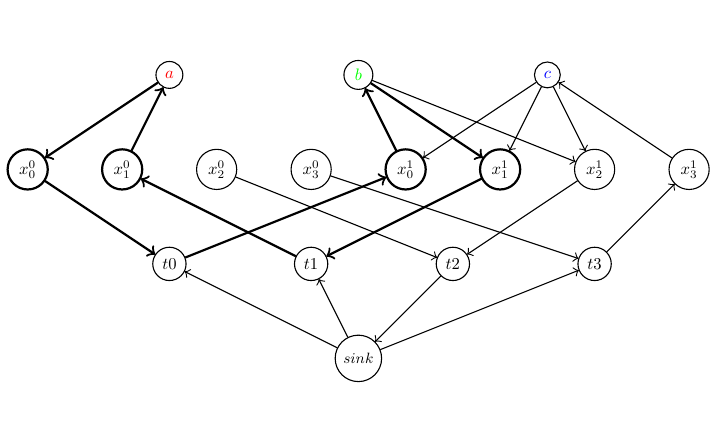
\begin{tikzpicture}[transform shape,scale=0.6]
      \useasboundingbox(0,0) rectangle (14,8);
      \tikzset{V/.style = {shape=circle, draw, text=black}}
      \tikzset{E/.style = {draw,text=black,->}}
      \node[V,text=red](d0) at (3,7) {$a$};
      \node[V,text=green](d1) at (7,7) {$b$};
      \node[V,text=blue](d2) at (11,7) {$c$};
      \node[V,thick](x00) at (0,5) {$x^0_0$};
      \node[V,thick](x01) at (2,5) {$x^0_1$};
      \node[V](x02) at (4,5) {$x^0_2$};
      \node[V](x03) at (6,5) {$x^0_3$};
      \node[V,thick](x10) at (8,5) {$x^1_0$};
      \node[V,thick](x11) at (10,5) {$x^1_1$};
      \node[V](x12) at (12,5) {$x^1_2$};
      \node[V](x13) at (14,5) {$x^1_3$};
      \node[V](t0) at (3,3) {$t0$};
      \node[V](t1) at (6,3) {$t1$};
      \node[V](t2) at (9,3) {$t2$};
      \node[V](t3) at (12,3) {$t3$};
      \node[V](t) at (7,1) {\small{$sink$}};
      \draw[E,thick](d0) to (x00);
      \draw[E,thick](x01) to (d0);
      \draw[E,thick] (x10) to (d1);
      \draw[E,thick](d1) to (x11);
      \draw[E](d1) to (x12);
      \draw[E](d2) to (x10);
      \draw[E](d2) to (x11);
      \draw[E](d2) to (x12);
      \draw[E](x13) to (d2);
      \draw[E,thick](x00) to (t0);
      \draw[E,thick](t0) to (x10);
      \draw[E,thick](t1) to (x01);
      \draw[E,thick](x11) to (t1);
      \draw[E](x02) to (t2);
      \draw[E](x12) to (t2);
      \draw[E](x03) to (t3);
      \draw[E](t3) to (x13);
      \draw[E](t) to (t0);
      \draw[E](t) to (t1);
      \draw[E](t2) to (t);
      \draw[E](t) to (t3);
    \end{tikzpicture}
  \end{figure}
  \begin{itemize}
  \item schedule: [ 1 0 -1 1 ] $\Rightarrow$ [ 0 1 -1 1 ]
  \end{itemize}
\end{frame}

\begin{frame}[fragile]
  \frametitle{Another simple directed cycle yielding another different schedule}
  \begin{figure}
    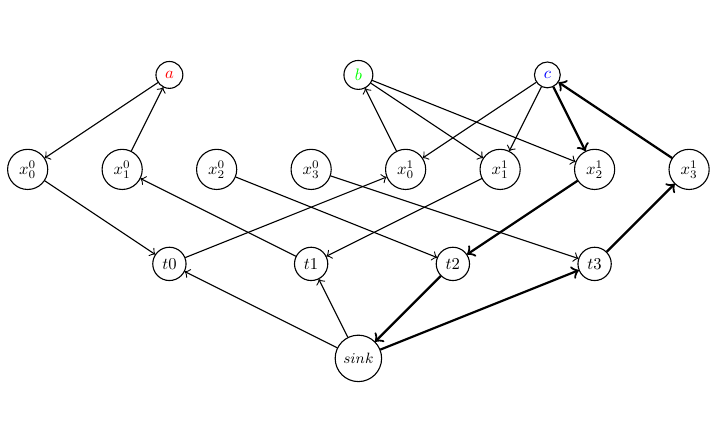
\begin{tikzpicture}[transform shape,scale=0.6]
      \useasboundingbox(0,0) rectangle (14,8);
      \tikzset{V/.style = {shape=circle, draw, text=black}}
      \tikzset{E/.style = {draw,text=black,->}}
      \node[V,text=red](d0) at (3,7) {$a$};
      \node[V,text=green](d1) at (7,7) {$b$};
      \node[V,text=blue](d2) at (11,7) {$c$};
      \node[V](x00) at (0,5) {$x^0_0$};
      \node[V](x01) at (2,5) {$x^0_1$};
      \node[V](x02) at (4,5) {$x^0_2$};
      \node[V](x03) at (6,5) {$x^0_3$};
      \node[V](x10) at (8,5) {$x^1_0$};
      \node[V](x11) at (10,5) {$x^1_1$};
      \node[V](x12) at (12,5) {$x^1_2$};
      \node[V](x13) at (14,5) {$x^1_3$};
      \node[V](t0) at (3,3) {$t0$};
      \node[V](t1) at (6,3) {$t1$};
      \node[V](t2) at (9,3) {$t2$};
      \node[V](t3) at (12,3) {$t3$};
      \node[V](t) at (7,1) {\small{$sink$}};
      \draw[E](d0) to (x00);
      \draw[E](x01) to (d0);
      \draw[E](x10) to (d1);
      \draw[E](d1) to (x11);
      \draw[E](d1) to (x12);
      \draw[E](d2) to (x10);
      \draw[E](d2) to (x11);
      \draw[E,thick](d2) to (x12);
      \draw[E,thick](x13) to (d2);
      \draw[E](x00) to (t0);
      \draw[E](t0) to (x10);
      \draw[E](t1) to (x01);
      \draw[E](x11) to (t1);
      \draw[E](x02) to (t2);
      \draw[E,thick](x12) to (t2);
      \draw[E](x03) to (t3);
      \draw[E,thick] (t3) to (x13);
      \draw[E] (t) to (t0);
      \draw[E] (t) to (t1);
      \draw[E,thick](t2) to (t);
      \draw[E,thick](t) to (t3);
    \end{tikzpicture}
  \end{figure}
  \begin{itemize}
    \item schedule: [ 1 0 -1 1 ] $\Rightarrow$ [ 1 0 1 -1 ]
  \end{itemize}
\end{frame}

\begin{frame}
  \frametitle{Algorithms for finding cycles}
  \begin{figure}
    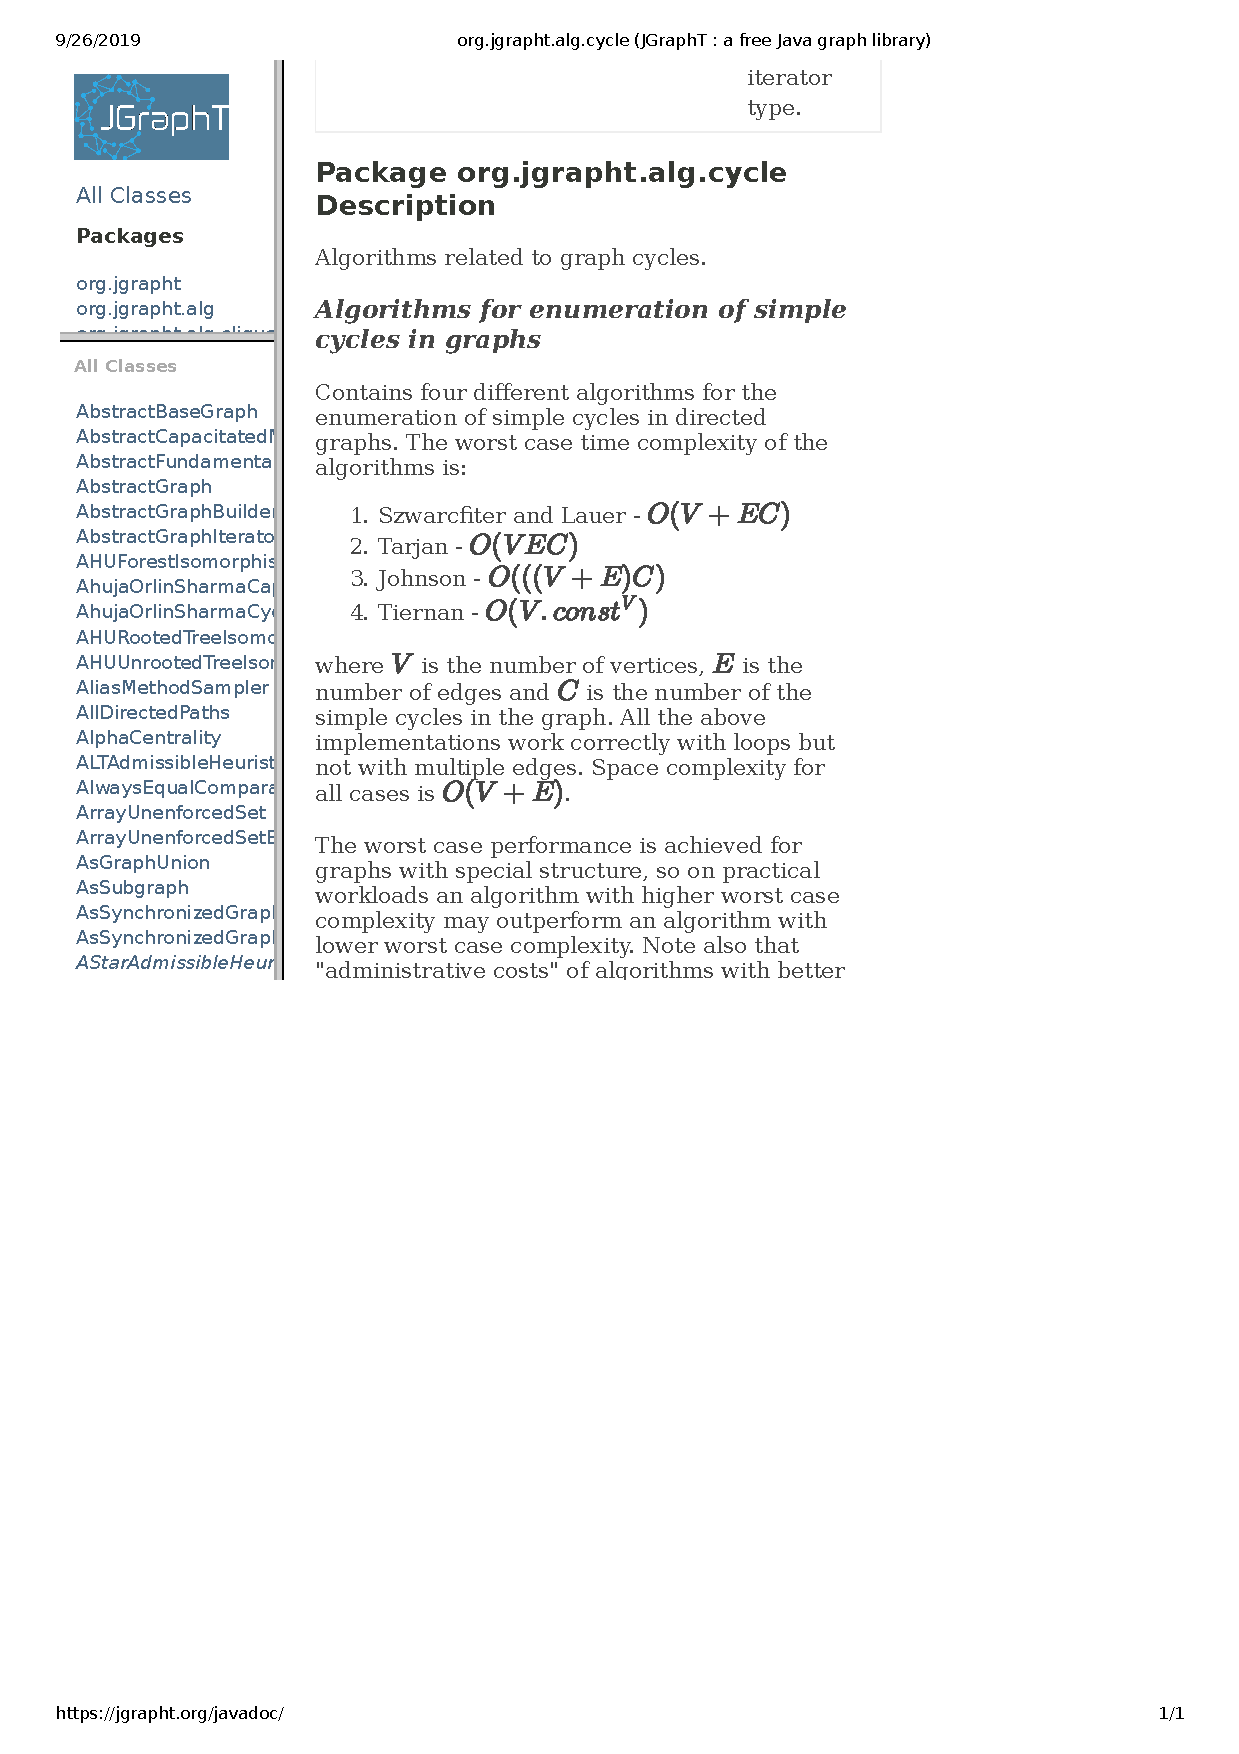
\includegraphics[width=0.8\textwidth]{jgrapht.pdf}
  \end{figure}
\end{frame}

\begin{frame}[fragile]
  \frametitle{Number of cycles grows exponentially in instance size}
\begin{figure}
\begin{minipage}{0.45\textwidth}
\footnotesize{\begin{verbatim}
15
5
0 0 0 0 0 0 0 0 1 0 0 0 0 0 0
0 0 0 0 0 0 0 0 0 1 0 0 1 0 0
0 0 0 0 0 0 0 0 0 0 1 0 0 0 0
0 0 0 0 0 0 0 0 0 0 0 0 0 1 0
0 0 0 0 0 0 0 0 0 1 1 0 0 0 0
10
0 78 86 93 120
165 0 193 213 178
214 170 0 190 185
178 177 185 0 196
201 199 215 190 0
\end{verbatim}
  }
\begin{itemize}
  \item 59118 cycles found in 0.359 seconds
\end{itemize}
\end{minipage}
\hfill
\begin{minipage}{0.45\textwidth}
  \footnotesize{\begin{verbatim}
  15
  6
  0 0 0 0 0 0 0 0 1 0 0 0 0 0 0
  0 0 0 0 0 0 0 0 0 1 0 0 1 0 0
  0 0 0 0 0 0 0 0 0 0 1 0 0 0 0
  0 0 0 0 0 0 0 0 0 0 0 0 0 1 0
  0 0 0 0 0 0 0 0 0 1 1 0 0 0 0
  0 0 0 0 0 0 0 0 0 0 1 0 0 0 1
  10
  0 78 86 93 120 12
  165 0 193 213 178 12
  214 170 0 190 185 12
  178 177 185 0 196 12
  201 199 215 190 0 12
  201 100 88 190 14 0
\end{verbatim}
  }
  \begin{itemize}
    \item 2646487 cycles found in 8.463 seconds
  \end{itemize}
\end{minipage}
\end{figure}
\end{frame}

\begin{frame}[fragile]
  \frametitle{Limit number of cycles by considering (different) subgraph(s)}
  \begin{figure}
      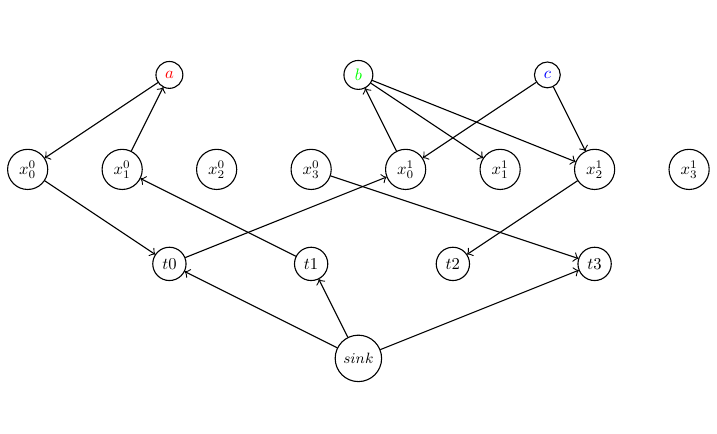
\begin{tikzpicture}[transform shape,scale=0.6]
      \useasboundingbox(0,0) rectangle (14,8);
      \tikzset{V/.style = {shape=circle, draw, text=black}}
      \tikzset{E/.style = {draw,text=black,->}}
      \node[V,text=red](d0) at (3,7) {$a$};
      \node[V,text=green](d1) at (7,7) {$b$};
      \node[V,text=blue](d2) at (11,7) {$c$};
      \node[V](x00) at (0,5) {$x^0_0$};
      \node[V](x01) at (2,5) {$x^0_1$};
      \node[V](x02) at (4,5) {$x^0_2$};
      \node[V](x03) at (6,5) {$x^0_3$};
      \node[V](x10) at (8,5) {$x^1_0$};
      \node[V](x11) at (10,5) {$x^1_1$};
      \node[V](x12) at (12,5) {$x^1_2$};
      \node[V](x13) at (14,5) {$x^1_3$};
      \node[V](t0) at (3,3) {$t0$};
      \node[V](t1) at (6,3) {$t1$};
      \node[V](t2) at (9,3) {$t2$};
      \node[V](t3) at (12,3) {$t3$};
      \node[V](t) at (7,1) {\small{$sink$}};
      \draw[E](d0) to (x00);
      \draw[E](x01) to (d0);
      \draw[E](x10) to (d1);
      \draw[E](d1) to (x11);
      \draw[E](d1) to (x12);
      \draw[E](d2) to (x10);
      \draw[E](d2) to (x12);
      \draw[E](x00) to (t0);
      \draw[E](t0) to (x10);
      \draw[E](t1) to (x01);
      \draw[E](x12) to (t2);
      \draw[E](x03) to (t3);
      \draw[E] (t) to (t0);
      \draw[E] (t) to (t1);
      \draw[E](t) to (t3);
      \end{tikzpicture}
  \end{figure}
\end{frame}

\begin{frame}
  \frametitle{Algorithmic idea}
  \begin{center}
  {\small
  \begin{algorithmic}[1]
    \State Compute initial feasible schedule $s$ 
    \State $\text{done} \gets \text{false}$
    \While{!done}
     \State Find set $C$ of directed cycles in (set of) residual subgraph(s)
     \State Compute best schedule $\bar{s}$ for $(C,s)$
     \If{cost($\bar{s}$) $<$ cost($s$)}
     \State $s \gets \bar{s}$
      \Else
      \State $\text{done} \gets \text{true}$
      \EndIf
     \EndWhile
  \end{algorithmic}
}
\end{center}
\end{frame}

\end{document}
